\chapter{Prompt Engineering}

\section{Azure OpenAI Access}
Microsoft instructions: \href{https://learn.microsoft.com/en-us/training/modules/get-started-openai/1-introduction}{Getting started with OpenAI}.

\section{Effective Prompts}
Effective system prompt:
\begin{numberedlist}
	\item Define the role.
	\item Define the objective/goal
	\item Any constraints/any specific rules
	\item Output format (bullet points, JSON, YAML)
\end{numberedlist} 

\section{Evaluation Metrics for Summarization}
\subsection{Introduction}
In order to evaluate model predictions (i.e., AI generated summaries), we compare the model predictions with the ground truth on a sample of human-annotated gold examples. However, given the subjective nature of model predictions, we need new metrics to evaluate summarization outputs: ROUGE and BERT Score.

\subsection{Recall-Oriented Understudy for Gisting Evaluation (ROUGE)}
What is ROUGE?
\begin{bulletedlist}
	\item ROUGE is a set of metrics that measure the similarity between a candidate summary and a set of reference summaries by comparing the grams (tokens, characters or words) present in them.
	\item The ROUGE score ranges from 0 to 1, with a score close to 1 indicating strong similarity between the candidate and reference summaries.
	\item Higher ROUGE scores indicate better performance in preserving key information from the original text while generating a concise summary
\end{bulletedlist}

Because it depends on the presence of exact matches, ROUGE is better fit for extractive summarization than abstractive.

\subsubsection{What is N-grams in ROUGE?}
\begin{bulletedlist}
	\item N-grams are a fundamental concept in Natural Language Processing (NLP). They are used to analyze and understand the structure of text by identifying sequences of n items (words, characters, or phonemes) from a given text.
	\item The term "n" in n-grams represents the size of the sequence (number of words), which can be any positive integer.
	\item ROUGE measure the overlap of n-grams between the system and reference summaries. N-grams refer to sequences of n items (words, characters, or phonemes) from a given text.
	\item The ROUGE metric is designed to capture the recall-oriented aspects of summarization, focusing on the ability of the generated summary to capture the essential information from the source text.
\end{bulletedlist}

\subsubsection{Types of ROUGE}
There are several variants of the ROUGE metric:
\begin{bulletedlist}
	\item ROUGE-N: Measures the overlap of n-grams (sequences of n words) between the system and reference summaries. For example, ROUGE-1 refers to the overlap of unigrams (single words), while ROUGE-2 refers to the overlap of bigrams (pairs of words).
	\item ROUGE-L: ROUGE-L, also known as ROUGE-LCS, focuses on the Longest Common Subsequence (LCS) between a system-generated summary and a reference summary. It aims to balance precision and recall by calculating a weighted harmonic mean, known as the F-measure.
	\begin{bulletedlist}
		\item LCS Importance: ROUGE-L considers the longest sequence of words shared between the system and reference summaries, allowing for non-consecutive matches that reflect sentence-level word order.
		\item Precision and Recall: It combines precision (correctness) and recall (completeness) to provide a comprehensive evaluation of summary quality.
	\end{bulletedlist}
	\item ROUGE-W: Both ROUGE-W and ROUGE-L are based on the longest common subsequence, while The key idea behind ROUGE-W is to assign higher weights to consecutive matches in the LCS, favoring summaries that maintain the order of words from the reference text.
	\item ROUGE-S is a metric used to evaluate the quality of automatically generated summaries by focusing on skip-bigrams. Skip-bigrams considers pairs of words that maintain their sentence order but may have other words in between, capturing the essence of sentence-level structure.
\end{bulletedlist}

\subsubsection{Example}
A common variant of ROUGE that is used to generate a comparison metric is ROUGE-L , where we first compute the recall and precision of the longest common subsequence and then compute the harmonic mean of these values (punctuation and case of the word are disregarded). 

 	\begin{figure}
		\centering
		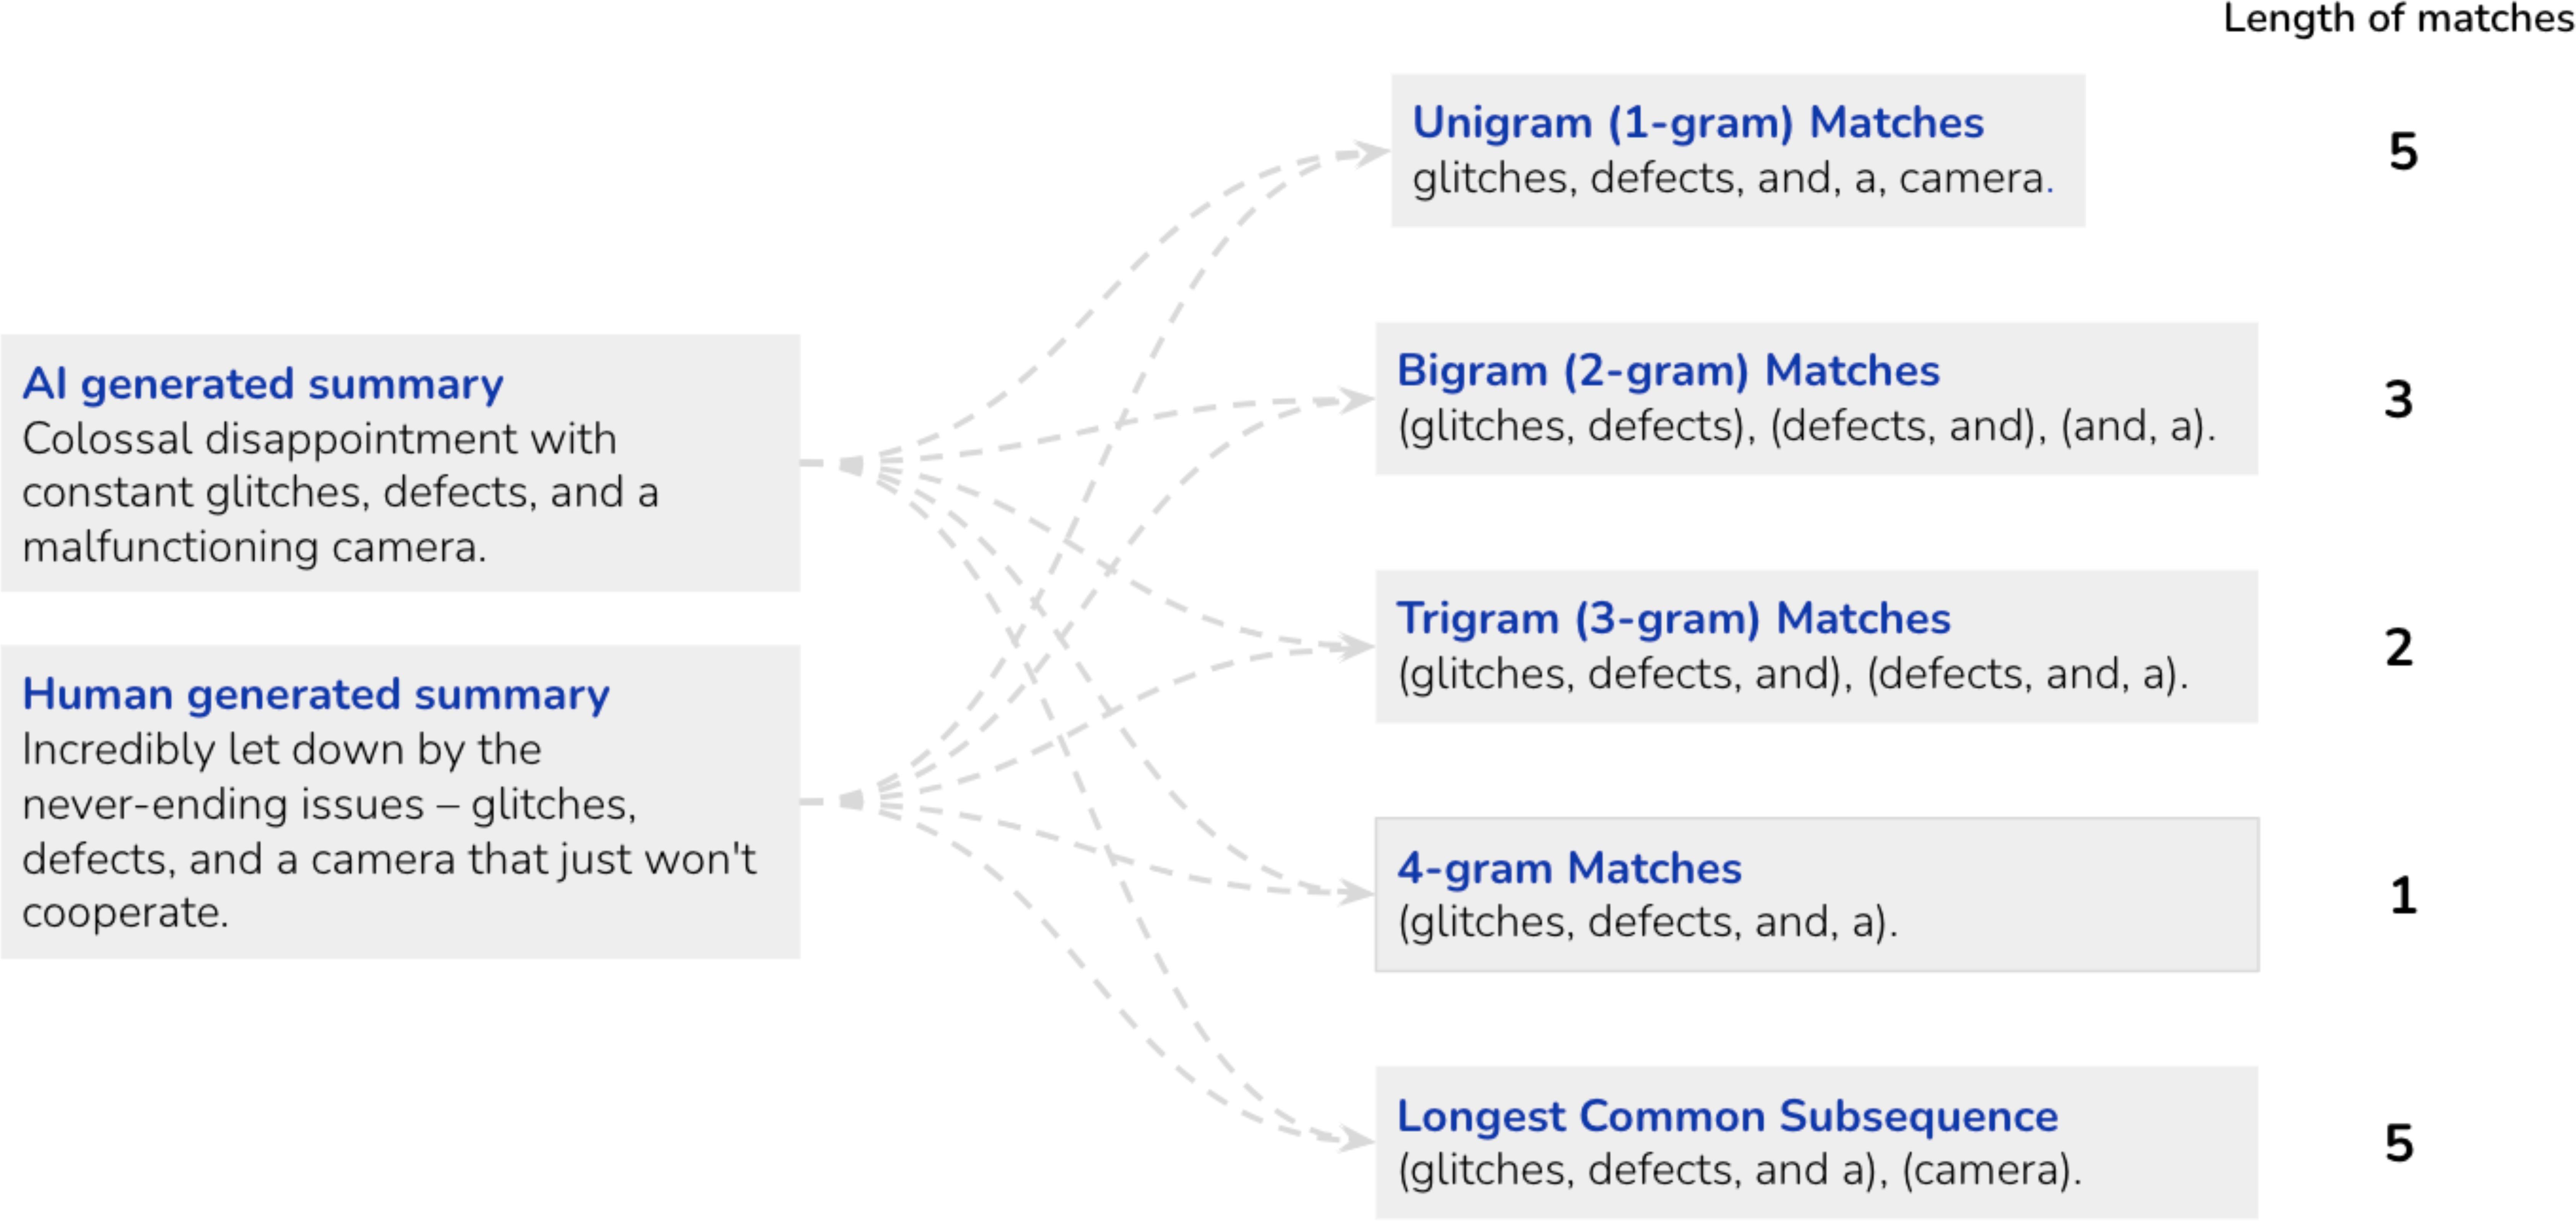
\includegraphics[width=5.0in]{summarizationmetricrouge}
		\caption[ROUGE N-grams]{ROUGE N-grams.}
		\label{fig:summarizationmetricrouge}
	\end{figure}


ai\_generated\_summary = "Colossal disappointment with constant glitches, defects, and a malfunctioning camera."
human\_generated\_summary = "Incredibly let down by the never-ending issues – glitches, defects, and a camera that just won't cooperate."

As seen in the figure above, the length of the largest common subsequence (LCS) between the two summaries is 5. The number of unigrams in the AI-generated summary is 10 and the number of unigrams in the human generated summary is 17.

We define the recall of the LCS as 5/17 and the precision of the LCS as 5/10 (notice the parallel with the precision and recall measures used to evaluate classification tasks).

From these measures, we can compute ROUGE-L as the F1 score associated with the precision and recall like so:

%r_lcs = 5/17
%p_lcs = 5/10
%
%(2 * r_lcs * p_lcs)/(r_lcs + p_lcs) # Rouge-L
 

ROUGE is effective in scenarios involving abstractive summarization tasks, automatic summarization evaluation, assessments of large language models (LLMs), and comparative analyses of different summarization approaches. However, ROUGE lacks semantic understanding and doesn't evaluate whether the system truly understood the meanings and concepts in the original text. This can be addressed by the next metrics which is BERT Score.

2. BERT Score
What is BERT Score?
The BERT Score is a novel automatic evaluation metric for text generation tasks, such as summarization, machine translation, and image captioning. It leverages the pre-trained contextual embeddings from BERT (Bidirectional Encoder Representations from Transformers) to measure the semantic similarity between the candidate (system-generated) and reference (ground truth) sentences.
Key Idea:

Embeddings: BERT Score uses the contextual embeddings from BERT to capture the semantic meaning of words in both the candidate and reference sentences.
Semantic Similarity: It computes the similarity between each word in the candidate sentence and each word in the reference sentence based on their contextual embeddings.
Precision, Recall, and F1 Score: BERT Score calculates precision, recall, and the F1 score based on the maximum similarity for each word, providing a comprehensive evaluation of the generated text
What are Embeddings in BERT Score?

Embeddings are a way for computers to understand the meaning of words based on the words around them. It's like when you read a sentence, you can figure out what a word means by looking at the other words in the sentence.

Example:

ai\_generated\_summary = "Major issues, malfunctioning camera."
human\_generated\_summary = "Severely disappointed, constant problems."
Look at the two summaries presented above. Though the choice of words is not exactly the same, both are close in intent.
In order to capture intent, we use specific models that encode the semantic meaning of words used in the models in a mathematical space where we can measure the distance between the words used.
Since distances can be computed, if two words are close to each other in this mathematical space (i.e., less distance), we can infer that these two words are close in meaning.
What are Embedding Models?

Models that encode the word mappings, that is, models that associate words with a list of numbers (called vectors) that define positions of the words in a mathematical space are referred to as embedding models. 
Embedding models are precursors to language models and are a crucial component of how we represent the semantic meaning of words used in text. For example, here glitches, problem and issues are the related words and will have similar representation in the model. 


So we can see that BERT Score provides a more nuanced evaluation by considering semantic similarity and context. However, BERT Score can be computationally intensive due to its reliance on pre-trained language models

\subsection{Conclusion}
In summary, both ROUGE and BERT Score have their strengths and weaknesses in evaluating text summarization systems. ROUGE offers a baseline for content selection, while BERT Score provides a more comprehensive assessment of semantic similarity and alignment with human judgments. The choice between the two metrics depends on the specific requirements of the summarization task and the desired level of granularity in the evaluation process. 